\documentclass{tietreport}
% Import images
\usepackage[final]{graphicx}
% Bibliography configuration
\usepackage[
  date=year,
  style=alphabetic,
  backend=biber,
  sorting=nty,
  maxnames=5,
  minnames=3,
  maxalphanames=4,
  minalphanames=3,
  backref=true,
  doi=false,
  isbn=false,
  url=false,
  eprint=false
]{biblatex}
\addbibresource{references.bib}
% Chapters open on the next available page rather than always a
% right-hand one, which is what was inserting blank filler pages.
\let\cleardoublepage\clearpage
%% ==================================================
%% CUSTOMIZE THESE FIELDS FOR YOUR PROJECT
%% ==================================================
% Course/Lab header
\TitlePageHeader{%
  UCS503P - Software Engineering Laboratory%
}
% Main project title
\ProjectTitle{%
  CampusXchange%
}
% Subtitle or project description
\ProjectSubTitle{%
  A Campus-Verified Marketplace for Selling,
  Lending, and Exchange%
}
% Student information (up to 4 students)
\author{%
  \texttt{1024030098} Garav Goyal \\
  \texttt{1024030102} Dhruv Rajput \\
  \texttt{1024030116} Parth Zutshi \\
  \texttt{1024030118} Harjap Singh Benipal%
}
% Group number, degree, year, program
\TitlePageSubText{%
  Group: \texttt{3C-14} BE Third Year, CSE%
}
% Faculty advisor/guide name
\AdvisorName{%
  Dr. Anushka%
}
% Evaluation period and department info
\TitlePageFooterText{{%
    \large Mid-Semester Evaluation \\[0.2cm]
    \bfseries Computer Science and Engineering
    Department%
  } \\[0.15cm]
  Thapar Institute of Engineering and Technology,
  Patiala%
}
%% ==================================================
\begin{document}
% Generate title page
\maketitle
% Table of contents (auto-generated from chapters)
\tableofcontents
% ===== CHAPTER 1: INTRODUCTION =====
\chapter{Introduction}
\section{Background and Context}
Campus commerce today runs on ad hoc, trust-optional
channels: hostel WhatsApp groups, batch chats, and the
occasional physical noticeboard. None of these were
designed for several hundred people who mostly do not
know each other to buy, sell, lend, or swap items
safely.

The inefficiency is not evenly spread across time. A
campus effectively re-runs the same shopping list every
semester: the same textbooks, calculators, drafters,
and lab coats change hands within a fixed population
that renews itself each year. That repetition means even
a modest improvement to trust and discoverability
compounds across thousands of small trades annually, in
a way it would not for a marketplace serving one-off
strangers.

\subsection{Problem Statement}
Four specific failures characterise the current
situation:

\begin{itemize}
  \item \textbf{No single place to look.} A listing
    lives in one hostel-wing group or one batch chat, so
    it rarely reaches anyone outside the poster's own
    circle. Buyers and sellers who would gladly trade
    never find each other.
  \item \textbf{Strangers with no proof.} Anyone can be
    added to these groups, including people with no
    genuine link to the college. There is no reliable
    way to confirm the other party is a current student
    before money or goods change hands.
  \item \textbf{Lending has no memory.} Every exchange
    is treated as a one-off sale. Nothing tracks who
    borrowed what, when it is due back, or whether a
    deposit was returned, so lending barely happens,
    despite being the natural fit for short-term items.
  \item \textbf{No recourse when it goes wrong.} If an
    item arrives damaged or a seller disappears after
    payment, there is no escrow, no verified handoff
    record, and no one to appeal to.
\end{itemize}

CampusXchange addresses these by building a mobile
marketplace in which identity is verified against the
institution, every listing is reviewed before publication,
and negotiation is recorded by the system rather than
left to informal chat.

\section{Project Objectives}
\begin{enumerate}
  \item \textbf{Verified access:} Restrict participation
    to holders of a valid \texttt{@thapar.edu} address,
    enforced in the database and not merely in the
    client, with each account additionally carrying a
    roll number and a manually reviewed student ID card.
  \item \textbf{Unified listing surface:} Provide a
    single searchable feed covering all three
    transaction types (Sell, Lend/Rent, and Exchange),
    filterable by category, replacing scattered
    group chats.
  \item \textbf{Moderated publication:} Ensure no listing
    reaches the public feed without passing through an
    administrative review queue, so trust and safety is
    a structural property of the system rather than a
    policy statement.
  \item \textbf{Recorded negotiation:} Move price
    agreement out of free-text conversation and into
    structured offers that the system stores, so that a
    concluded deal has an auditable record.
  \item \textbf{Complete system model:} Produce a full
    UML specification of the system (including the
    transaction, handoff, and dispute phases scheduled
    after this evaluation), so that implementation of
    the remaining modules proceeds from a validated
    design.
\end{enumerate}

These objectives are deliberately scoped so that each is
independently demonstrable at the mid-semester
evaluation, with the remaining transaction core designed
and modelled but explicitly deferred.

% ===== CHAPTER 2: METHODOLOGY & DESIGN =====
\chapter{Methodology and Design}
\section{System Architecture}
CampusXchange follows a three-tier architecture: a
mobile client, a stateless backend API, and a managed
data platform. A deliberate design decision separates
two paths through the system: authentication traffic
goes directly from the client to the identity provider,
while all application data is mediated by the backend.

\subsection{High-Level Design}
Figure~\ref{fig:architecture} shows the system as
currently built. Boxes drawn solid are implemented and
verified; those drawn dashed are designed but not yet
coded.

\begin{figure}[h]
  \centering
  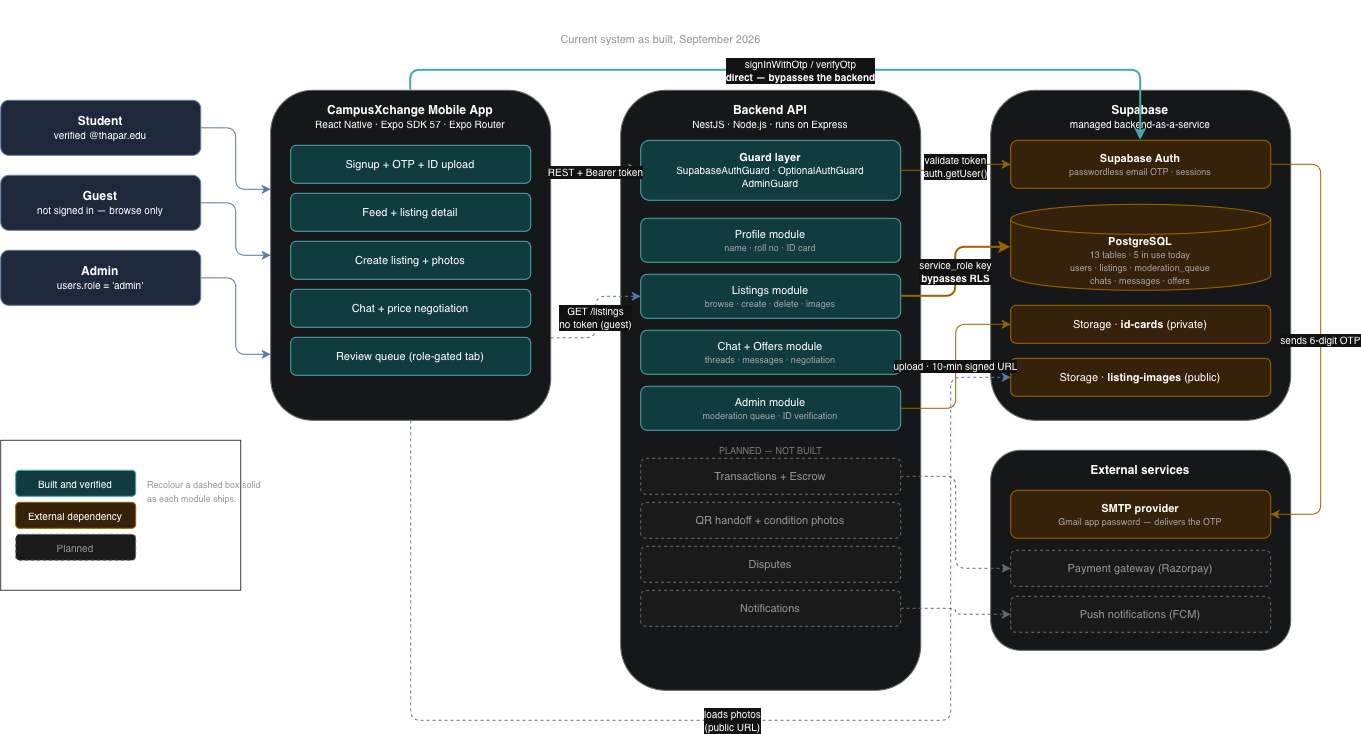
\includegraphics[width=\textwidth]{figures/architecture-highlevel.png}
  \caption{High-level system architecture. Solid
    components are implemented; dashed components are
    designed and scheduled for the next phase.}
  \label{fig:architecture}
\end{figure}

The major components interact as follows:

\begin{itemize}
  \item \textbf{Mobile client.} The only user-facing
    surface. It serves three classes of user: a
    verified student, a guest who may browse but not
    act, and an administrator whose additional review
    screen is unlocked by a role flag on their account.
  \item \textbf{Authentication path.} The client calls
    the identity provider directly to request and verify
    a one-time password. The backend is not involved in
    this exchange; it only ever receives the resulting
    session token. This keeps credential handling
    entirely outside our own code.
  \item \textbf{Backend API.} A stateless service
    organised into feature modules, fronted by a guard
    layer that validates every incoming request before
    any business logic executes. Three guards exist: one
    requiring a valid session, one that permits
    anonymous access while still identifying a caller if
    a token is present, and one that additionally
    requires an administrator role.
  \item \textbf{Data platform.} A managed PostgreSQL
    instance plus two object-storage buckets. The
    separation of the buckets is a security decision:
    student ID cards are held privately and reached only
    through short-lived signed URLs issued to
    administrators, whereas listing photographs are
    public because every browsing user, including
    guests, must be able to load them.
\end{itemize}

Two aspects of Figure~\ref{fig:architecture} deserve
particular attention. First, the backend holds a
privileged database key that bypasses row-level security;
this is why that key never ships inside the mobile
application. Second, guest browsing is served by the
same endpoint as authenticated browsing: the backend
detects the absence of a token and withholds the meeting
location from the response, so an unauthenticated user
can see what is for sale but not where the exchange
would take place.

\subsection{Technical Stack}
\begin{itemize}
  \item \textbf{Framework/Language:} React Native with
    Expo (SDK 57) and Expo Router for the mobile client;
    NestJS on Node.js for the backend API. TypeScript
    throughout, giving a single type vocabulary across
    both tiers.
  \item \textbf{Database:} PostgreSQL, provisioned
    through Supabase. Thirteen tables model the complete
    system; five are exercised by the code delivered so
    far.
  \item \textbf{Tools:} Git and GitHub for version
    control, with a GitHub Actions workflow that
    type-checks the mobile application and compiles the
    backend on every push; draw.io for UML modelling;
    Expo Go for on-device testing.
  \item \textbf{Libraries:} Supabase client libraries for
    authentication, database access and object storage;
    \texttt{class-validator} for request validation at
    the API boundary; \texttt{expo-image-picker} and
    \texttt{expo-file-system} for photograph capture and
    upload.
\end{itemize}

\subsection{System Modelling and UML Diagrams}
The system was specified using four UML diagram types
before and alongside implementation. Together they
answer four different questions: what the system does
(use case), what data it holds (class), what messages
are exchanged (sequence), and what the workflow is
(activity). Every diagram covers the complete proposed
system, including the modules deferred past this
evaluation, so that the deferred work proceeds from a
validated design rather than from scratch.

\subsubsection{Use Case Diagram}
Figure~\ref{fig:usecase} identifies four actors and
nineteen use cases. The actors are Student, Verified
Student, Administrator, and an external Notification
Service.

\begin{figure}[h]
  \centering
  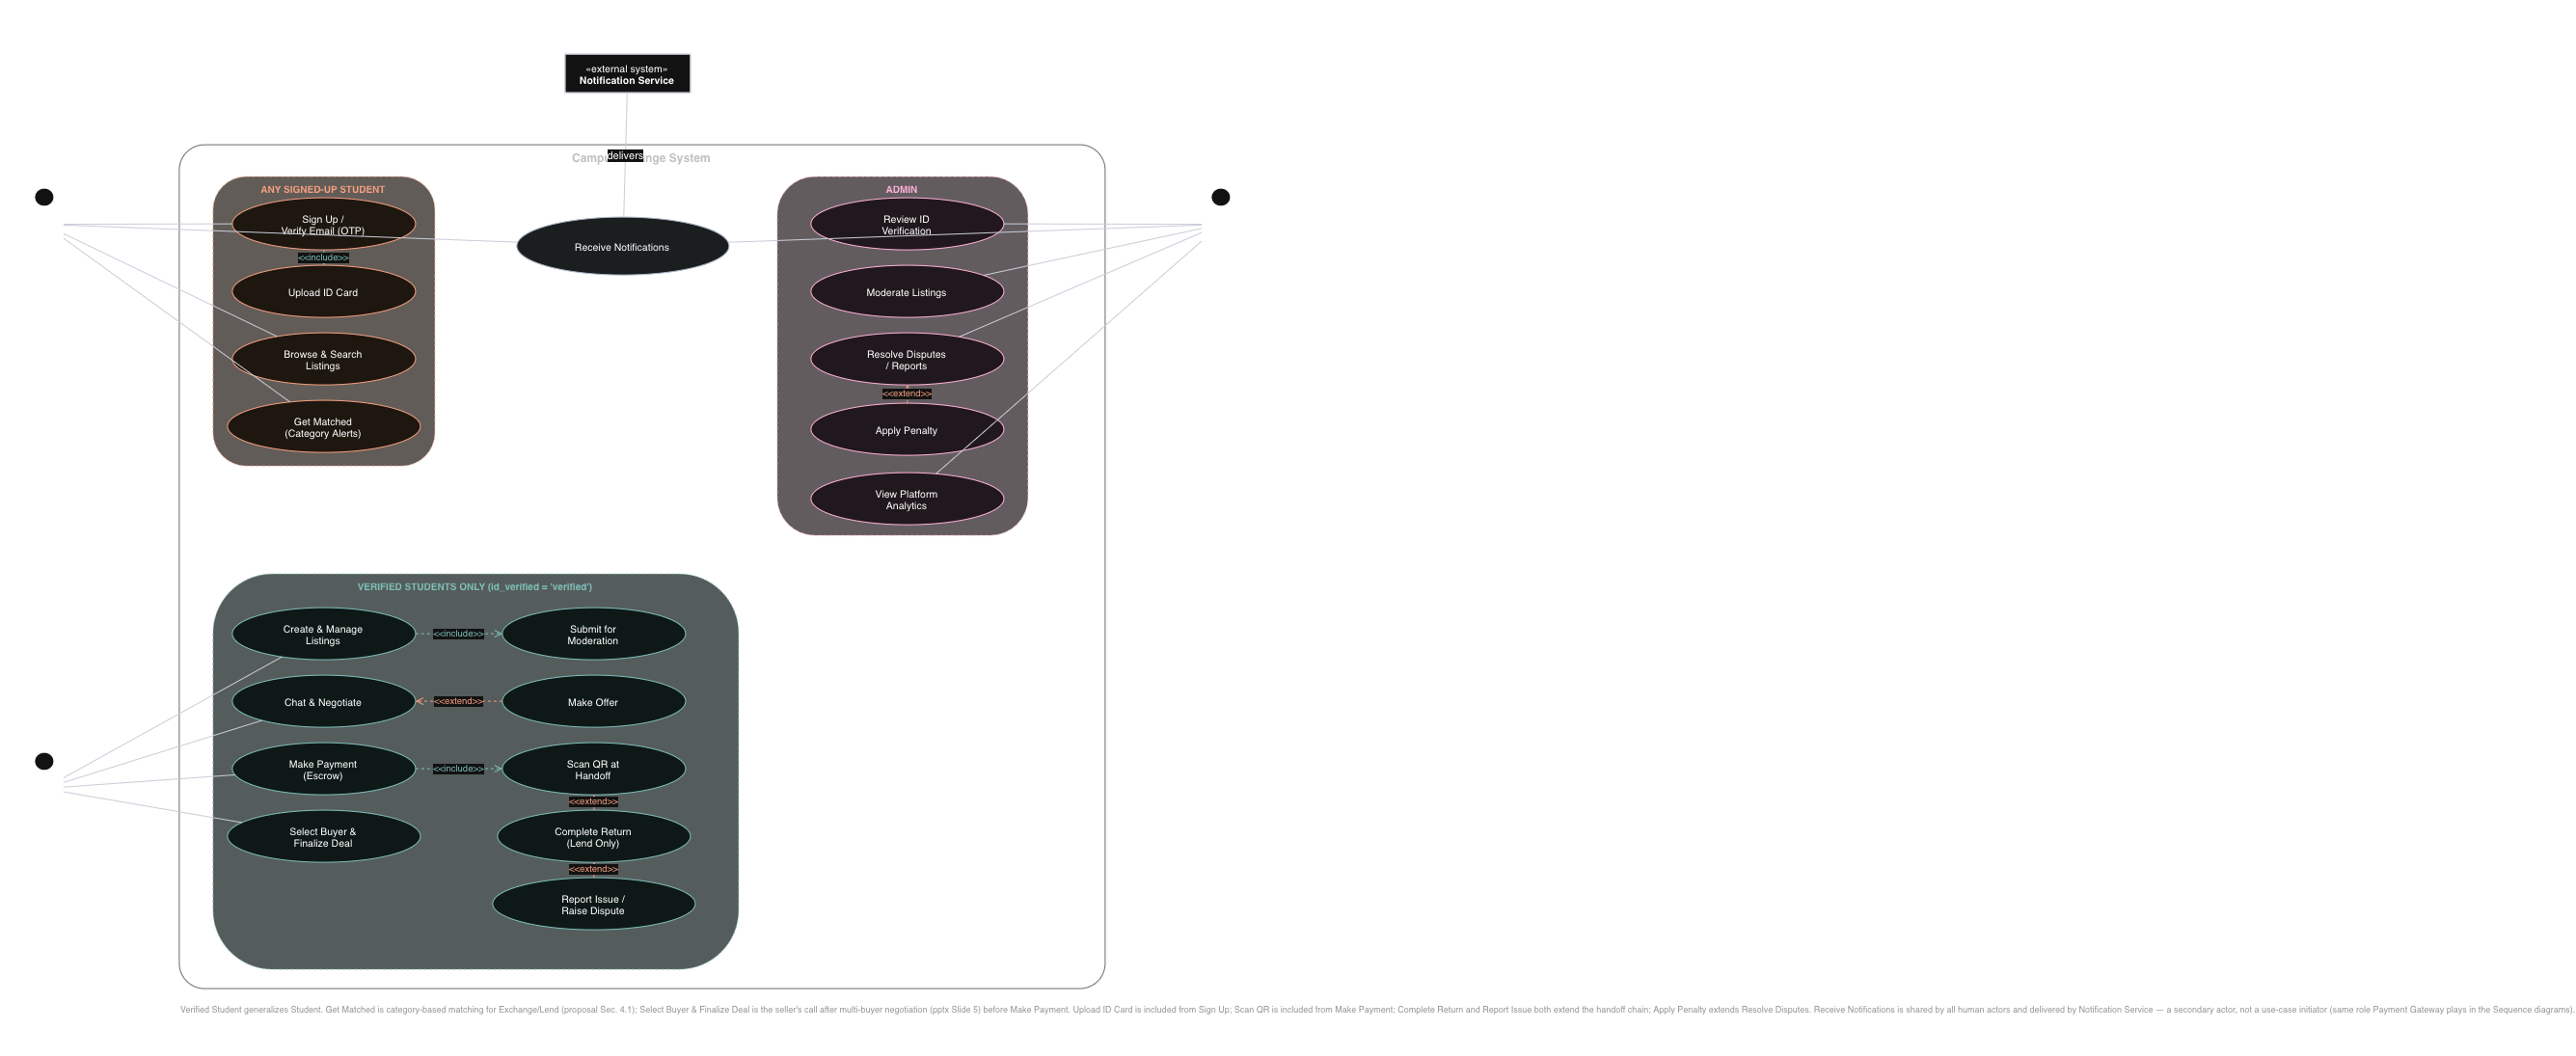
\includegraphics[width=\textwidth]{figures/usecase.png}
  \caption{Use case diagram: four actors and nineteen
    use cases, partitioned by privilege level.}
  \label{fig:usecase}
\end{figure}

The important structural feature is the partition into
privilege bands. A merely signed-up Student may sign up,
upload an ID card, browse, and receive category alerts.
Only a Verified Student, one whose ID card has been
approved by an administrator, may create listings,
negotiate, pay, or raise a dispute. Verified Student
generalises Student, so the second band inherits
everything in the first. This is the diagram-level
expression of the project's central claim: that
verification is a gate, not a badge.

The Notification Service is modelled as a secondary
actor. It receives output from the system but never
initiates a use case, which is the same relationship the
Payment Gateway holds in the sequence diagrams.

\subsubsection{Class and Entity-Relationship Diagram}
Figure~\ref{fig:class} presents all thirteen tables with
their full columns and constraint flags, generated
directly from the live database schema.

\begin{figure}[h]
  \centering
  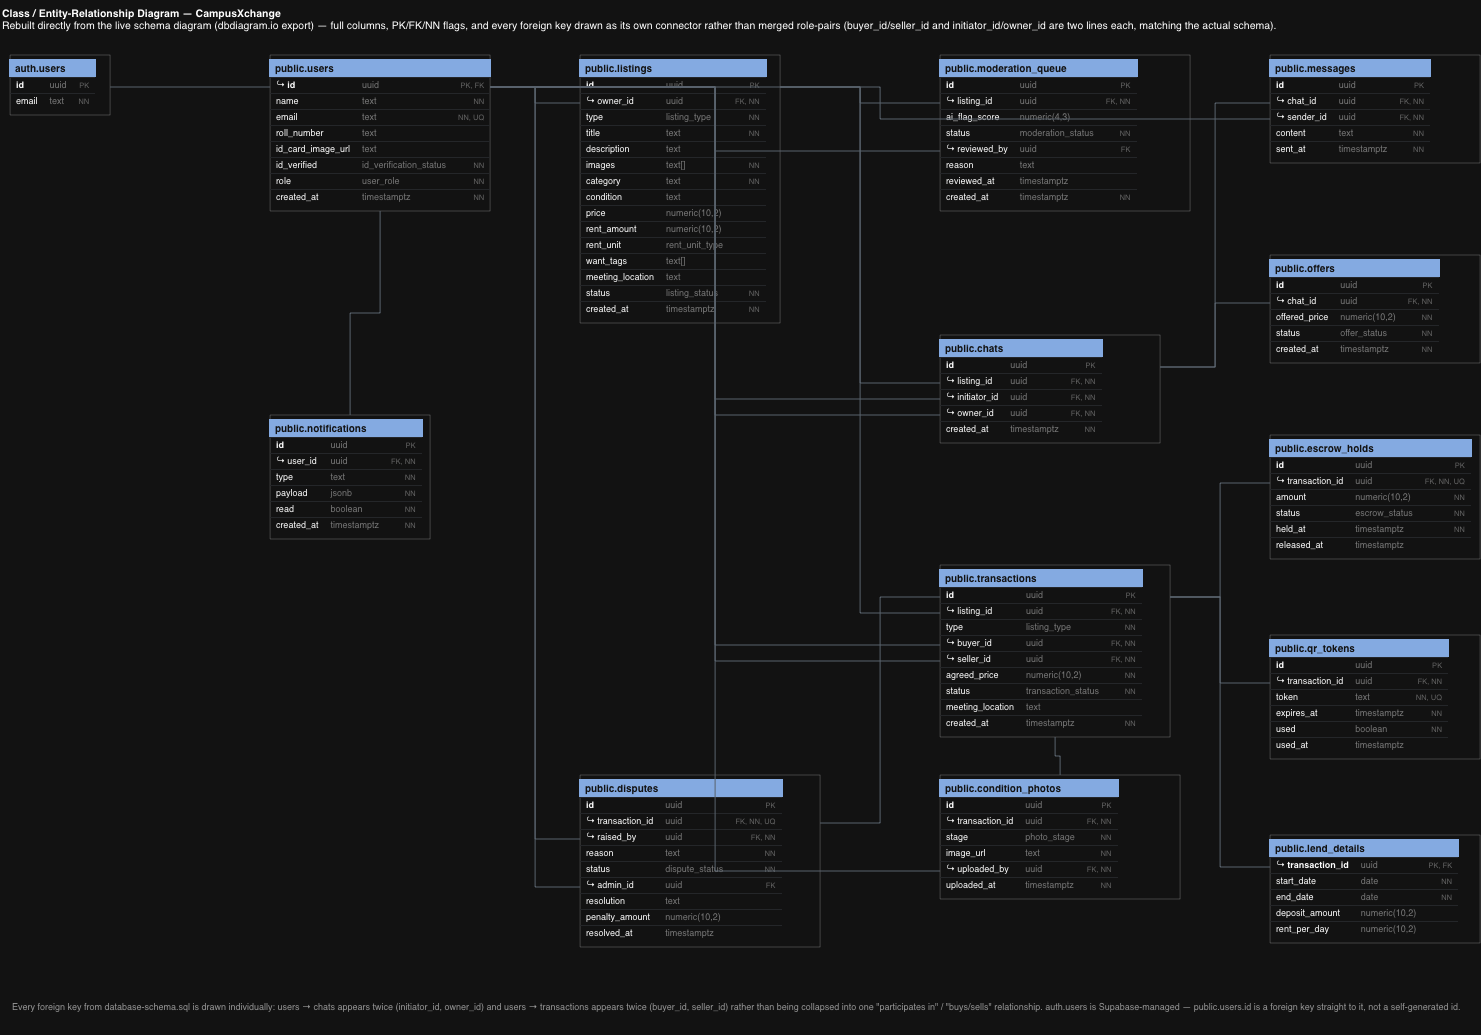
\includegraphics[width=\textwidth]{figures/class-er.png}
  \caption{Class / entity-relationship diagram: thirteen
    tables with primary, foreign and not-null
    constraints.}
  \label{fig:class}
\end{figure}

Two modelling decisions are worth drawing out. First,
\texttt{public.users} is not the source of identity:
its primary key is a foreign key to the
authentication provider's own user table. Our table is a
profile that extends an identity owned elsewhere, and a
database trigger creates that profile row automatically
the moment an account is created. Second, every foreign
key is drawn as its own connector rather than being
merged into a conceptual relationship: \texttt{chats}
references \texttt{users} twice (as initiator and as
owner), and \texttt{transactions} references it twice
again (as buyer and as seller). Collapsing these into a
single ``participates in'' line would have hidden the
fact that the two roles are separately constrained.

\subsubsection{Sequence Diagrams}
The sequence model is one continuous diagram spanning
three pages, connected by labelled off-page connectors.
It traces the full lifetime of a transaction at the
level of individual messages between participants.

\begin{figure}[h]
  \centering
  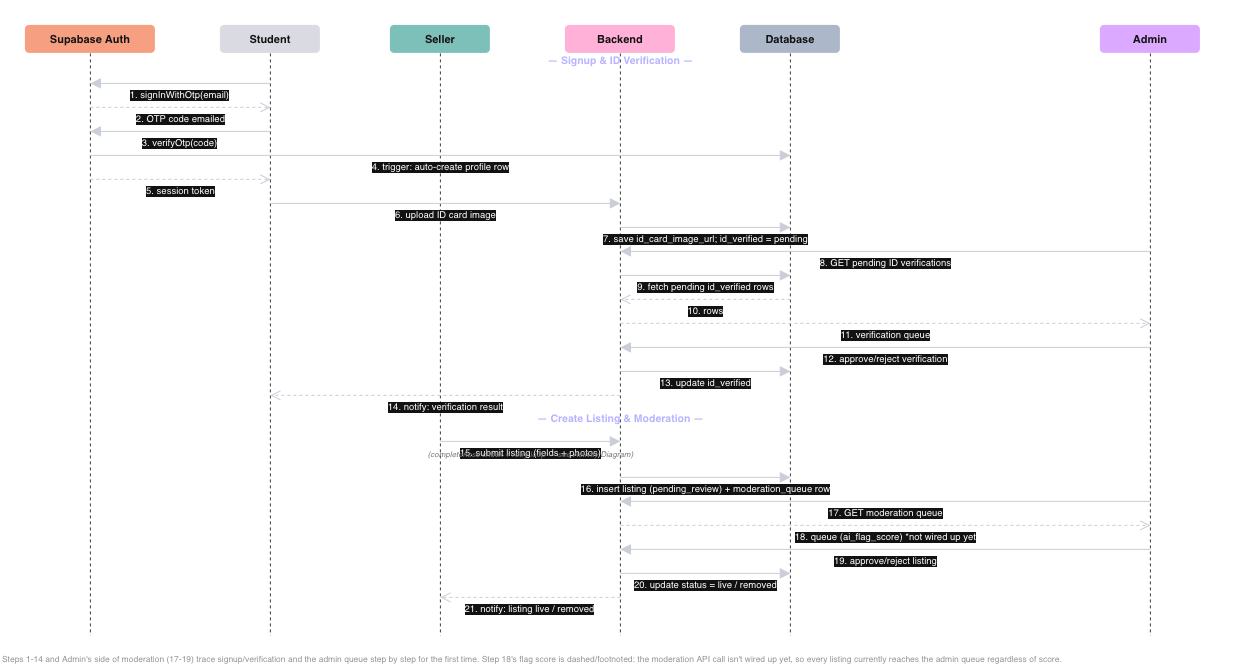
\includegraphics[width=\textwidth]{figures/sequence-1-signup-moderation.png}
  \caption{Sequence diagram (1 of 3): signup, ID
    verification, listing creation and moderation.}
  \label{fig:seq1}
\end{figure}

Figure~\ref{fig:seq1} covers signup and moderation.
Steps~1--5 show the one-time password exchange happening
between the student and the authentication provider
directly, with the database receiving an automatically
triggered profile row rather than an explicit insert
from our backend. Steps~8--13 show the administrator's
side of ID verification. Step~18 is drawn dashed: the
automated content-flag score is not wired up, so in the
delivered system every listing reaches the human review
queue regardless of score.

\begin{figure}[h]
  \centering
  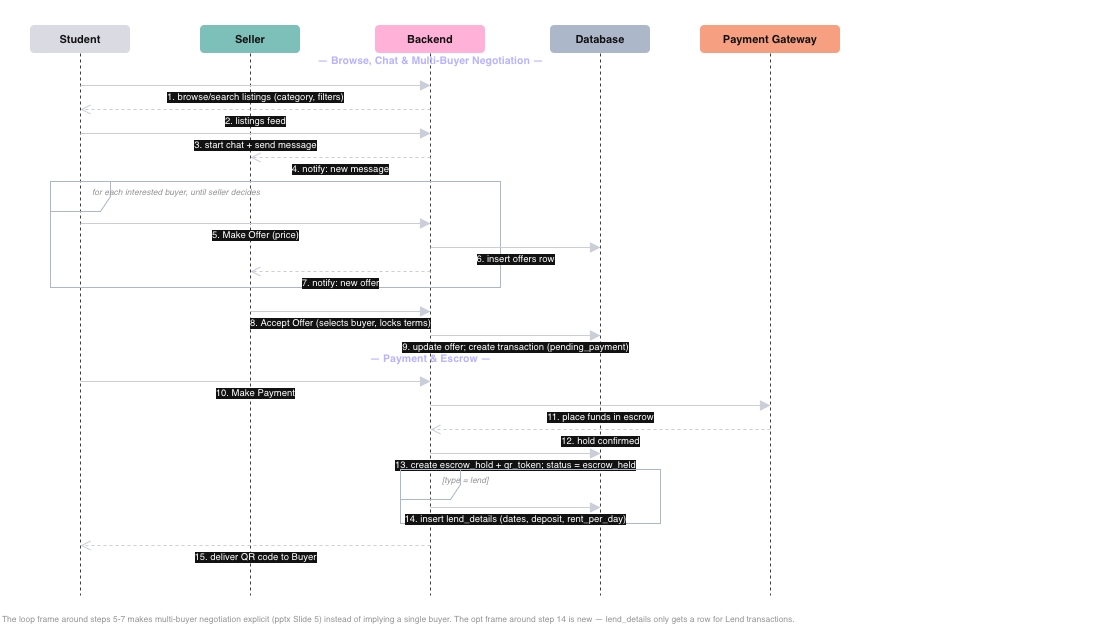
\includegraphics[width=\textwidth]{figures/sequence-2-negotiation-payment.png}
  \caption{Sequence diagram (2 of 3): browsing, chat,
    multi-buyer negotiation, payment and escrow.}
  \label{fig:seq2}
\end{figure}

Figure~\ref{fig:seq2} covers negotiation. The
\texttt{loop} fragment around steps~5--7 is significant:
it makes explicit that several buyers may be negotiating
on the same listing concurrently, and that the seller
chooses between them. A diagram without that fragment
would have implied a single buyer and quietly designed
out the competition the marketplace depends on. The
\texttt{opt} fragment at step~14 records that lend-specific
terms are stored only for lend transactions.

\begin{figure}[h]
  \centering
  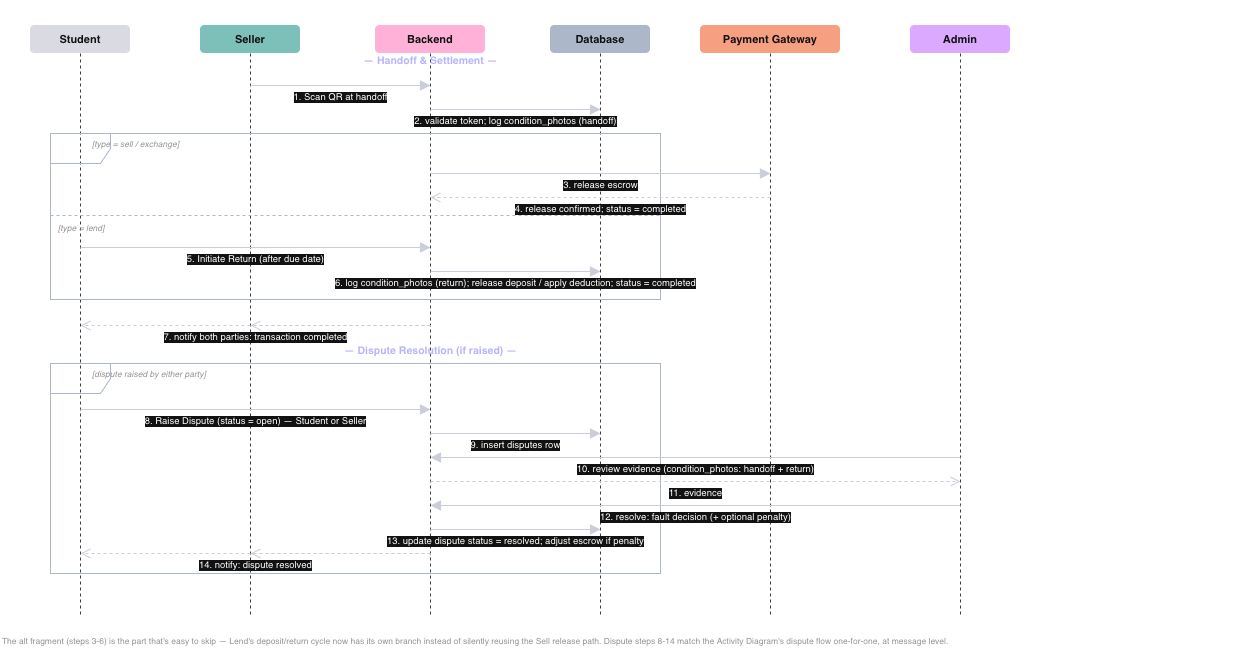
\includegraphics[width=\textwidth]{figures/sequence-3-handoff-disputes.png}
  \caption{Sequence diagram (3 of 3): QR-verified
    handoff, settlement and dispute resolution.}
  \label{fig:seq3}
\end{figure}

Figure~\ref{fig:seq3} covers handoff and settlement. The
\texttt{alt} fragment separates the sell and exchange
path, where escrow releases immediately on a valid QR
scan, from the lend path, which additionally requires a
return leg with its own condition photographs before the
deposit is settled. Modelling these as alternatives
rather than reusing the sell path prevented a real design
error: a borrowed item would otherwise have been
marked complete at handoff, before it was returned.

\subsubsection{Activity Diagrams}
The activity model mirrors the same three phases at the
level of decisions and control flow rather than
messages. Where the sequence diagrams answer ``who sends
what to whom,'' these answer ``what is decided, and what
happens on each branch.''

\begin{figure}[h]
  \centering
  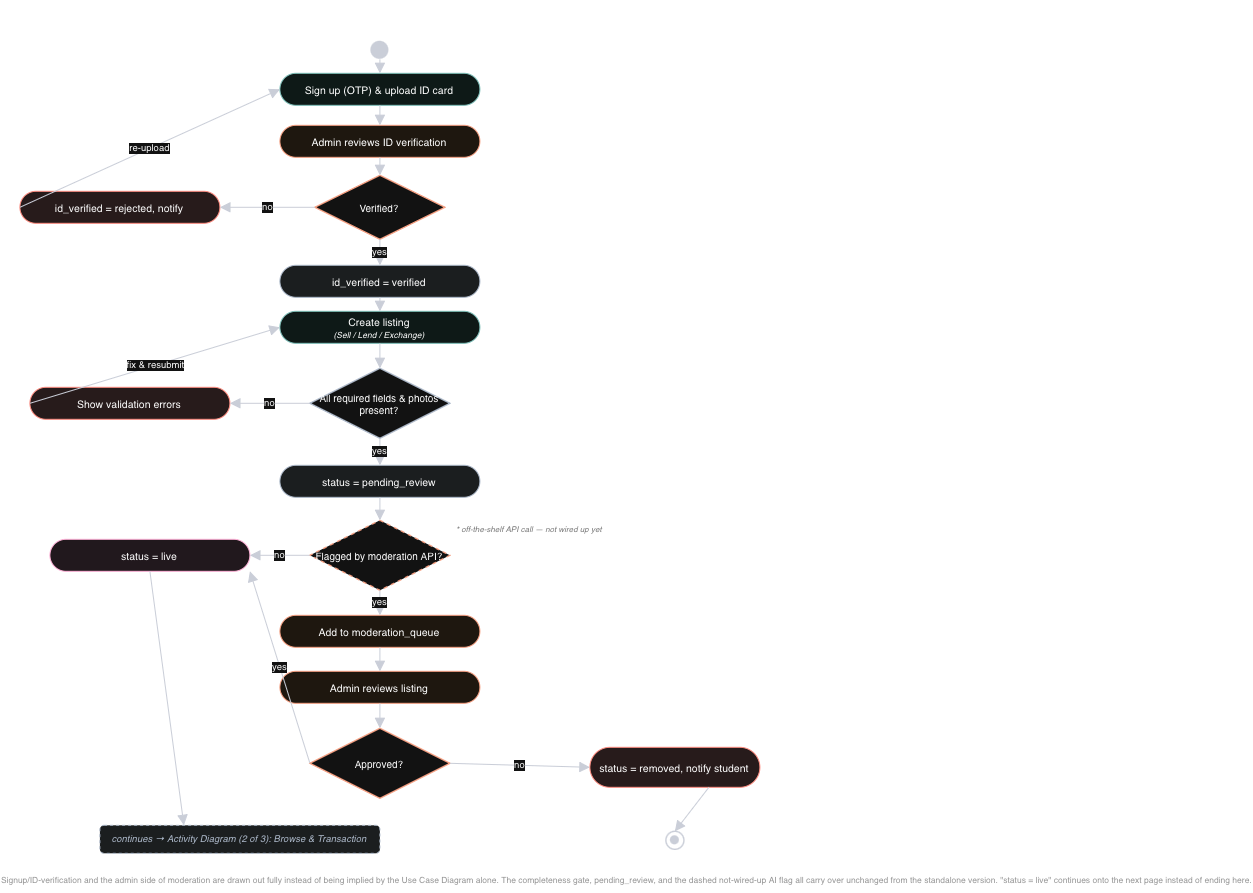
\includegraphics[width=0.86\textwidth]{figures/activity-1-signup-moderation.png}
  \caption{Activity diagram (1 of 3): verification and
    moderation, showing both rejection loops.}
  \label{fig:act1}
\end{figure}

Figure~\ref{fig:act1} shows two rejection loops that a
purely happy-path design would have missed: a rejected
ID card returns the student to re-upload, and a listing
failing the completeness check returns to the form with
validation errors. Only after both gates does a listing
reach \texttt{pending\_review}, and only administrator
approval moves it to \texttt{live}.

\begin{figure}[h]
  \centering
  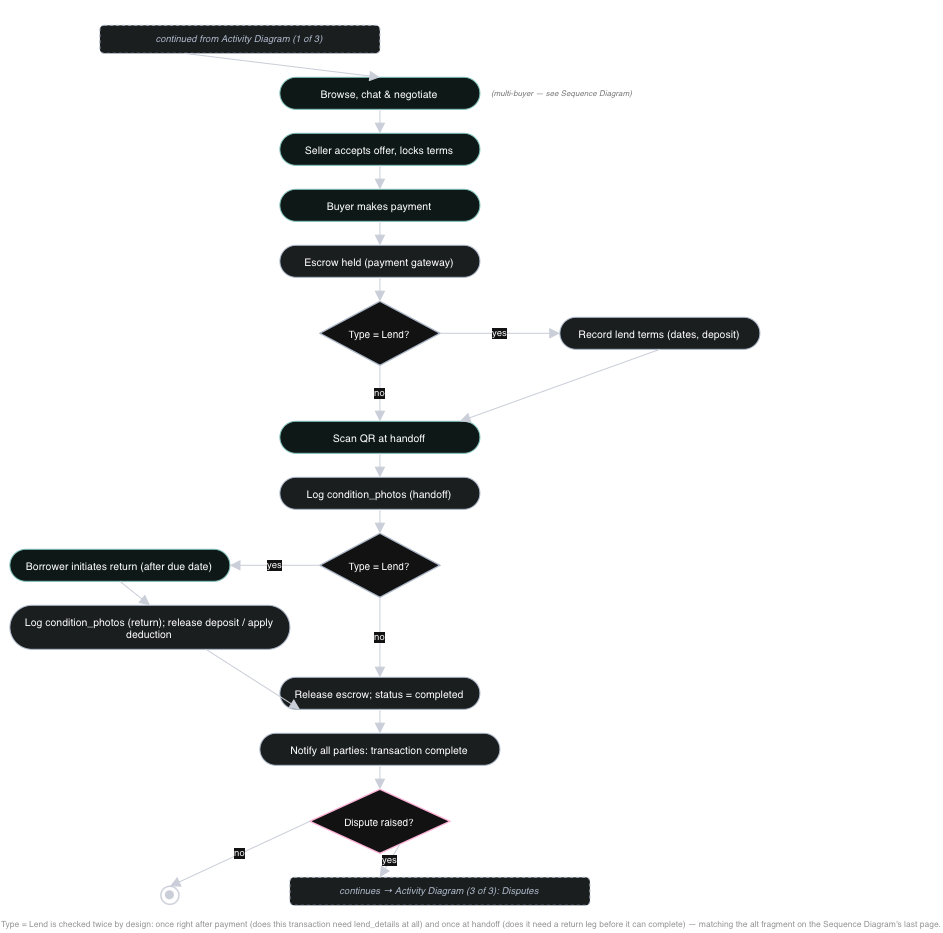
\includegraphics[width=0.72\textwidth]{figures/activity-2-transaction.png}
  \caption{Activity diagram (2 of 3): negotiation,
    payment, handoff and the lend return cycle.}
  \label{fig:act2}
\end{figure}

In Figure~\ref{fig:act2} the transaction type is tested
twice, and deliberately so. The first test, immediately
after payment, asks whether lend-specific terms need to
be recorded at all. The second, at handoff, asks whether
a return leg must complete before the transaction can
close. The two questions are distinct, occur at
different times, and merging them would have produced
the same defect the sequence model avoided.

\begin{figure}[h]
  \centering
  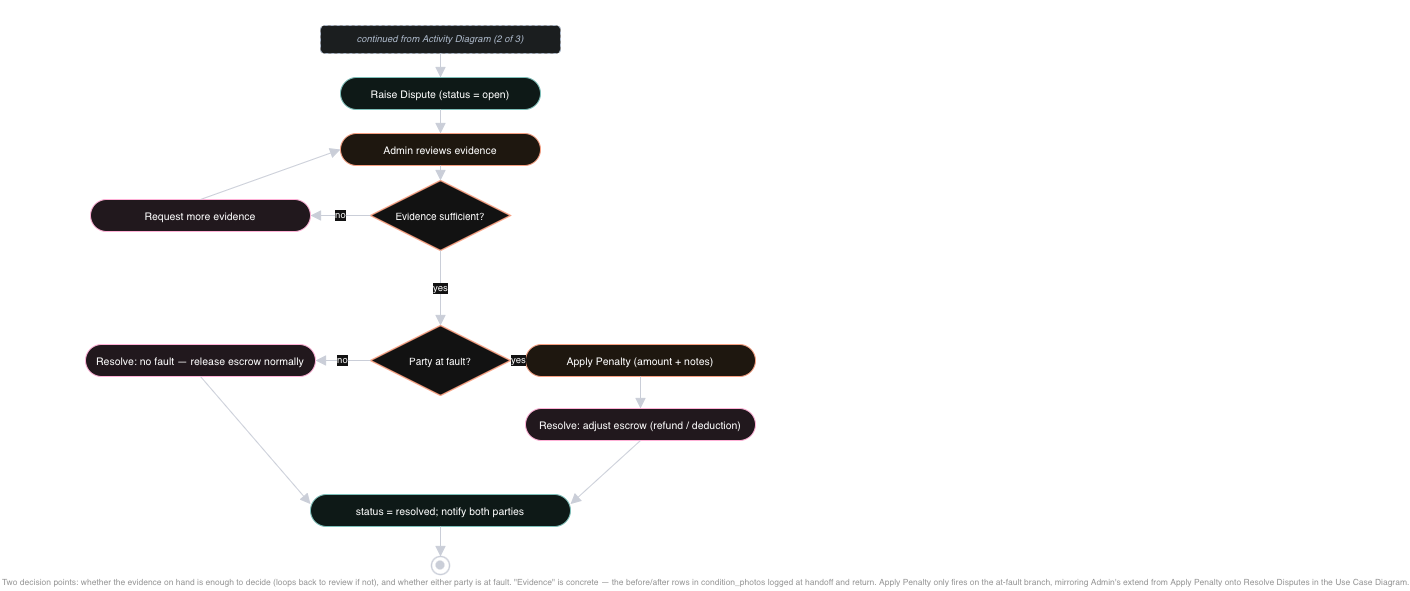
\includegraphics[width=\textwidth]{figures/activity-3-disputes.png}
  \caption{Activity diagram (3 of 3): dispute
    resolution and penalty application.}
  \label{fig:act3}
\end{figure}

Figure~\ref{fig:act3} models dispute resolution around
two decisions: whether the available evidence is
sufficient to decide, which loops back to review if it
is not, and whether either party is at fault. The
evidence in question is concrete: the before-and-after
condition photographs captured at handoff and return,
which is what makes an adjudicated outcome possible at
all.

\section{Implementation Details}
\subsection{Module 1: Verified Access and Identity}
Identity is deliberately not built in-house. Signup uses
a passwordless one-time password flow provided by the
authentication service, which removes password storage,
hashing and reset flows from our threat surface
entirely.

Restricting signup to the institution required work at
two levels. The client validates the address before
requesting a code, but a client-side check is
cosmetic: a modified application, or a direct call to
the public API, bypasses it. The enforcement that matters
is a database trigger which raises an exception on any
account whose address does not end in the institutional
domain, aborting the insert transaction so that no
account is created and no code is ever sent.

The second identity component is the student ID card.
The photograph is uploaded through the backend to a
private bucket, namespaced by user so that no student can
overwrite another's file, and the profile is marked
awaiting review. An administrator later approves or
rejects it. There is no optical character recognition or
third-party document-verification vendor; a human makes
the decision, which is both simpler and more defensible
than an unvalidated automated classifier.

\subsection{Module 2: Listings and Moderation}
A listing is a single entity with three type-specific
shapes. Rather than three tables, one table carries a
type discriminator and the columns relevant to each
type: a price for sell, a rent amount and unit for
lend, a set of wanted tags for exchange. The API
validates that the fields required by the declared type
are present, so a sell listing without a price is
rejected at the boundary.

Moderation is enforced structurally. Creation writes the
listing at \texttt{pending\_review} and simultaneously
inserts a row into the moderation queue; the public feed
query returns only listings at \texttt{live}. A student
therefore cannot publish directly, and this is a
property of the data flow rather than of a rule that
could be forgotten. The two writes are coupled: if the
queue insert fails, the listing is rolled back, so the
two tables cannot disagree about whether an item is
awaiting review.

\subsection{Module 3: Chat and Structured Negotiation}
Conversation is scoped to one thread per interested buyer
per listing, enforced by a uniqueness constraint. Access
is checked on every message operation: a caller who is
neither party to a thread receives a forbidden response.

The negotiation layer is what distinguishes this from a
messaging application. An offer is a first-class record
carrying a price, a status, and the identity of the party
who proposed it. Either party may propose; only the
other party may accept or reject, which is enforced in
the service rather than the interface. Accepting one
offer automatically rejects all other pending offers on
that thread, so a thread cannot arrive at two
simultaneously agreed prices. Once any offer is
accepted, the thread is closed to further offers.

The client merges messages and offers into a single
timeline ordered by timestamp, so a negotiation reads in
the order it actually happened.

\subsection{Module 4: Administrative Review}
The administrative surface is delivered inside the mobile
application as a tab that appears only for accounts
carrying the administrator role. It presents two queues:
listings awaiting moderation, and student ID cards
awaiting verification.

The role check on the client controls only the tab's
visibility. Authorisation is enforced server-side by a
guard that re-reads the caller's role from the database
on every administrative request, so modifying the
application to reveal the tab would not grant access to
any administrative operation.

Because the ID-card bucket is private, the review screen
cannot simply link to an image. The backend issues a
signed URL valid for ten minutes per card, so
administrators can view exactly what they need to review
and nothing persists as a shareable link afterwards.

% ===== CHAPTER 3: RESULTS & EVALUATION =====
\chapter{Results and Evaluation}
\section{Testing Methodology}
Verification at this stage was functional and
structural rather than performance-oriented; the system
has not yet been deployed or subjected to concurrent
load, so latency and throughput figures would not be
meaningful. The following were carried out:

\begin{itemize}
  \item \textbf{Static verification:} The entire mobile
    codebase type-checks under the TypeScript compiler
    in strict mode, and the backend compiles cleanly.
    Both checks run automatically on every push through
    a GitHub Actions workflow, so a change that breaks
    either is caught before review.
  \item \textbf{Build verification:} The mobile
    application was bundled for Android on every
    significant change, confirming that all modules
    resolve and that no dependency is missing from the
    dependency graph.
  \item \textbf{Authorisation testing:} Every protected
    endpoint was exercised without a token, and with a
    deliberately invalid token, confirming rejection in
    each case. Guest-accessible endpoints were verified
    to succeed without a token while still withholding
    the meeting location.
  \item \textbf{Integration testing:} The moderation
    loop was exercised end to end on a real device:
    create a listing, observe it held at
    \texttt{pending\_review} and absent from the public
    feed, approve it from the administrative queue, and
    observe it appear.
  \item \textbf{User testing:} Conducted informally
    within the project group on physical devices over a
    shared network. Several defects surfaced this way
    that static checks could not have caught, discussed
    in Section~3.3.
\end{itemize}

\section{Delivered Functionality}
Table~\ref{tab:delivered} summarises the status of each
module against the original proposal.

\begin{table}[h]
\centering
\begin{tabular}{|l|c|}
  \hline
  \textbf{Module} & \textbf{Status} \\
  \hline
  Verified signup (OTP + roll number + ID) & Implemented \\
  \hline
  Domain restriction (database-enforced) & Implemented \\
  \hline
  Listing feed, search, category filter & Implemented \\
  \hline
  Guest browsing (location withheld) & Implemented \\
  \hline
  Listing creation, all three types & Implemented \\
  \hline
  Photograph upload & Implemented \\
  \hline
  Moderation queue and review & Implemented \\
  \hline
  Administrative ID verification & Implemented \\
  \hline
  Chat and structured negotiation & Implemented \\
  \hline
  Payments and escrow & Designed \\
  \hline
  QR-verified handoff & Designed \\
  \hline
  Lend return and disputes & Designed \\
  \hline
  Push notifications & Designed \\
  \hline
\end{tabular}
\caption{Module delivery status at mid-semester
  evaluation. ``Designed'' denotes fully modelled in UML
  with database support present, but not yet
  implemented.}
\label{tab:delivered}
\end{table}

Nine of thirteen modules are implemented. Five of the
thirteen database tables are exercised by delivered
code; the remaining eight support the deferred
transaction core and already exist, so no schema
migration will be required when that work begins.

\section{Analysis}
\textbf{Objectives met.} Objectives~1 through~4 are
fully met. Verified access is enforced at the database
level rather than only in the client; the unified feed
covers all three transaction types; no listing can reach
the public feed without administrative approval; and
negotiation produces structured, stored offers rather
than free text. Objective~5 is met in full: the complete
system, including the deferred modules, is specified
across the diagrams presented in Section~2.1.3.

\textbf{Where the work exceeded the plan.} Guest
browsing was not in the original proposal. It emerged
from the use case model, which showed browsing available
to any signed-up student, and was extended so that
unauthenticated visitors can evaluate the marketplace
before committing to verification. The privacy
concern this raised, that meeting locations would
become publicly visible, was resolved by withholding
that single field server-side rather than by abandoning
the feature.

\textbf{Challenges encountered.} Three are worth
recording.

\begin{itemize}
  \item \textbf{Framework-level file upload failure.}
    Image upload failed consistently with an opaque
    error. The cause was that the mobile framework had
    replaced the standard network primitive with its own
    implementation, which rejects the conventional
    file-attachment format. Resolution required reading
    the framework's own source to determine the accepted
    shape, then adopting its file abstraction.
  \item \textbf{Silent build failure.} The backend build
    tool was configured to clear its output directory
    before compiling. When that step failed, the build
    reported success while leaving stale output in place,
    so newly added routes appeared to compile but
    returned not-found at runtime. Diagnosis required
    inspecting the compiled output rather than trusting
    the build's exit status.
  \item \textbf{Authentication email delivery.} The
    platform's built-in mail service is rate-limited and,
    for newer projects, does not permit template
    customisation, meaning verification emails
    contained a link rather than the numeric code our
    flow expects. Resolution required configuring an
    external mail provider and rewriting both email
    templates.
\end{itemize}

Each of these was a defect in an assumption about a
dependency rather than in our own logic, which is itself
a finding: the integration points, not the application
code, consumed the majority of debugging effort.

% ===== CHAPTER 4: CONCLUSION =====
\chapter{Conclusion}
\section{Summary of Work}
We set out to build a campus-verified marketplace in
which identity is checked against the institution, every
listing is reviewed before publication, and price
agreement is recorded by the system. At the mid-semester
point, that core is working: a student signs up with an
institutional address and a one-time code, supplies a
roll number and an ID card photograph, and browses a
feed covering all three transaction types. They can post
an item with photographs and a campus meeting point,
which enters a moderation queue and appears publicly
only once an administrator approves it. They can open a
conversation on any listing and negotiate through
structured offers until a price is agreed.

Alongside the implementation, the complete system (including
payments, QR-verified handoff, and dispute
resolution) has been specified across four UML diagram
types, so the remaining work proceeds from a validated
design.

\section{Key Findings}
\begin{itemize}
  \item \textbf{Finding 1:} Enforcing a constraint in the
    interface is not enforcing it at all. The
    institutional-domain restriction, the administrator
    role check, and the ownership check on deletion each
    began as client-side logic and each had to be moved
    into the database or the API guard layer before it
    became a real guarantee.
  \item \textbf{Finding 2:} Modelling caught design
    errors that implementation would have shipped. The
    lend return cycle, drawn as an alternative branch in
    the sequence and activity models, revealed that
    reusing the sell settlement path would have marked
    borrowed items complete at handoff, before their
    return.
  \item \textbf{Finding 3:} Integration cost dominated.
    The three most time-consuming defects all arose at
    boundaries with external dependencies (the mobile
    framework's network layer, the backend build tool,
    and the authentication provider's mail service)
    rather than within our own logic.
  \item \textbf{Finding 4:} Structural enforcement of
    moderation proved simpler than a policy. Because the
    feed query filters on published status and creation
    writes an unpublished one, there is no code path
    through which an unreviewed listing can become
    visible.
\end{itemize}

\section{Future Work and Recommendations}
\begin{enumerate}
  \item \textbf{Complete the transaction core.}
    Implement escrow, QR-verified handoff, condition
    photographs and the lend return cycle. The schema and
    the models already exist; this is implementation
    against a settled design~\cite{latex2e}.
  \item \textbf{Enable row-level security.} All tables
    are currently unrestricted. Because the client never
    queries tables directly and the backend holds a
    privileged key, policies can be enabled without
    altering application behaviour, and it should be done
    before any wider release.
  \item \textbf{Replace polling with real-time
    transport.} Chat currently refreshes on a fixed
    interval. A socket-based transport would reduce both
    latency and unnecessary requests.
  \item \textbf{Deploy the backend.} The API presently
    runs locally, which constrains testing to a shared
    network. A hosted deployment would allow genuine
    multi-user testing and, in turn, the performance
    measurement absent from this report.
  \item \textbf{Proximity-aware discovery.} The proposal
    envisaged ordering the feed by nearness to the
    viewer's hostel. Listings already record a meeting
    point; the viewer's own location is not yet stored,
    and adding it would complete the feature.
\end{enumerate}

\section{Final Remarks}
The most instructive lesson of this phase concerned
where trust actually lives in a software system. Every
safety property the proposal promised (that users are
real students, that listings are reviewed, that only the
owner can remove a listing) was straightforward to
express in the interface and consistently harder to
guarantee underneath it. In each case the version that
held was the one enforced closest to the data.

The second lesson concerned the value of modelling
ahead of code. The diagrams in this report were not
documentation produced after the fact; they exposed
branches, loops and failure paths that the
implementation would otherwise have discovered late, and
the deferred half of the system is consequently in a
position to be built from a specification rather than
from assumption.

% ===== BIBLIOGRAPHY =====
% Print bibliography with heading in TOC
\printbibliography[heading=bibintoc]
\end{document}
